\documentclass[11pt]{article}
\usepackage[margin=1in]{geometry}
\usepackage[T1]{fontenc}
\usepackage{lmodern}
\usepackage{microtype}
\usepackage{graphicx}
\usepackage{booktabs}
\usepackage{amsmath}
\usepackage{xcolor}
\usepackage[hidelinks]{hyperref}
\usepackage{enumitem}
\setlist{nosep, leftmargin=*}
\emergencystretch=3em

\newcommand{\repo}{\url{https://github.com/Tar-ive/trn1-llm-roofline}}

\title{How Close Does LLM Inference Get to the Hardware Limit\\on a Single AWS Trainium1 Chip?\\[0.4em]
\large A \$6 roofline study of TinyLlama-1.1B and Llama-3.1-8B on \texttt{trn1.2xlarge}}
\author{Saksham Adhikari}
\date{Technical report, November 2026 \\ \small Not peer reviewed. Code, raw results and run logs: \repo}

\begin{document}
\maketitle

\begin{abstract}
We measure prefill and decode latency of two Llama-architecture models on the smallest Trainium1 instance
(\texttt{trn1.2xlarge}: one chip, two NeuronCore-v2, 32\,GB HBM) with AWS NxD Inference on Neuron SDK 2.28,
and compare each phase with a simple hardware floor: HBM bandwidth for decode, dense BF16 throughput for prefill.
At batch 1 with tensor parallelism 2, decode reaches 54\% of the bandwidth floor for TinyLlama-1.1B and 63\% for
Llama-3.1-8B; prefill reaches 34\% and 59\% of the compute floor. Efficiency rises with model size because fixed per-step
costs are amortized over more bytes and FLOPs. Splitting even a 1.1B model across both cores decodes 1.9$\times$ faster than
one core, despite the cross-core all-reduce. Batching Llama-3.1-8B from 1 to 16 sequences yields 12$\times$ the decode tokens/s
for 34\% more step time. Serving TinyLlama through vLLM adds roughly 55\% to the per-token latency of NxD Inference's raw decode
step. All runs used self-terminating instances; total compute cost was about \$6. We describe the measurement pipeline and the
practical obstacles (SDK support for Trn1 ends at 2.28; compile time dominates a one-hour budget) and list the limits of a study
with one run per configuration.
\end{abstract}

\section{Motivation}
Accelerator datasheets give peak FLOPs and bandwidth, but practitioners choosing hardware need to know what fraction of those
peaks an off-the-shelf inference stack delivers. LLM inference has two phases with different limits: \emph{prefill} processes the
whole prompt in large matrix multiplies and is compute-bound, while \emph{decode} produces one token per sequence per step and must
stream every weight from HBM each step, so at small batch it is bandwidth-bound~\cite{williams2009roofline,pope2023efficiently}.
We ask a narrow question: on the cheapest Trainium1 instance, with AWS's own inference library and no custom kernels, how far is
each phase from its floor, and what moves it?

\section{Hardware and software}
\textbf{Hardware.} \texttt{trn1.2xlarge} has one Trainium1 chip with two NeuronCore-v2 cores sharing 32\,GB of HBM at about
820\,GB/s, and roughly 190 dense BF16 TFLOPS for the chip. Each core has a 128$\times$128 systolic matrix engine (TensorE), vector
and scalar engines, a 24\,MB on-chip SBUF scratchpad, and DMA engines. The host has 8 vCPUs and about 30\,GiB of usable RAM.
On-demand price in \texttt{us-east-1} was \$1.34/hour.

\textbf{Software.} Neuron SDK 2.29 and later removed Trn1 support from NxD Inference and \texttt{vllm-neuron}; our first run on the
latest Deep Learning AMI (SDK 2.33) failed for that reason. All results use the Neuron 2.28 DLAMI (2026-02-27):
\texttt{neuronx-cc} 2.23.6484, NxD Inference (NxDI) 0.8.16251, \texttt{torch-neuronx} 2.9.0, runtime 2.30.51, driver 2.26.5,
vLLM 0.13 with \texttt{vllm-neuron} 0.4.1.

\textbf{Models.} TinyLlama-1.1B-Chat (2.20\,GB in BF16) and Llama-3.1-8B-Instruct (16.06\,GB). 8B is the largest dense BF16 model
that leaves room for a KV cache on this chip; a 14B model ($\approx$28\,GB) would not.

\section{Method}
\textbf{Floors.} With $W$ the weight bytes, $P = W/2$ the parameter count, $T$ the prompt length and $B$ the batch size:
\begin{align*}
t_\text{decode} &\ge \frac{W}{\text{820\,GB/s}} &
t_\text{prefill} &\ge \frac{2PTB}{\text{190\,TFLOPS}}
\end{align*}
The decode floor counts weights only (it ignores KV-cache reads); the prefill floor counts only the $2P$ FLOPs per token of the
linear layers (it ignores attention FLOPs). Both floors are therefore optimistic, and the reported efficiencies are lower bounds on
how well the hardware is used. For TinyLlama the floors are 2.68\,ms per decode step and 5.93\,ms per 512-token prefill; for
Llama-3.1-8B, 19.59\,ms and 86.56\,ms per 1024-token prefill.

\textbf{Measurement.} NxDI's \texttt{inference\_demo --benchmark} compiles one graph for context encoding (prefill) and one per
token-generation bucket (decode), then runs 20 full generations and reports p50 and p99 latency per graph. We report p50;
p99 was within 1\% of p50 in every configuration. Sampling ran on device (top-$k$ = 1). TinyLlama used a 512-token prompt and
1024-token sequence; Llama-3.1-8B used 1024 and 2048. Device profiles were captured with the Neuron runtime inspector and summarized
with \texttt{neuron-profile}. Serving was measured with \texttt{vllm bench serve} (random prompts, 256 tokens in, 128 out, 64 prompts)
against one server, at client concurrency 1 and 4.

\textbf{Pipeline.} Each run launches a self-terminating instance that clones the repository, runs the benchmark script, and pushes
results to git after every step and every 10 minutes, with a hard power-off at the time budget. Llama-3.1-8B was compiled on a
CPU-only \texttt{m7i.4xlarge} (target override to Trn1) and the compiled artifacts cached in S3, so the Trainium instance only
downloaded them (15--16\,GB in about 90\,s per variant) instead of compiling on its 8 vCPUs.

\section{Results}

\begin{table}[t]
\centering
\small
\setlength{\tabcolsep}{4pt}
\begin{tabular}{lrrrrrrr}
\toprule
Model & TP & Batch & Prefill ms & \% peak & Decode ms & \% HBM BW & Decode tok/s \\
\midrule
TinyLlama-1.1B & 1 & 1  & 24.9   & 24 & 9.26  & 29 & 108 \\
TinyLlama-1.1B & 1 & 4  & 118.3  & 20 & 9.93  & 27 & 403 \\
TinyLlama-1.1B & 2 & 1  & 17.5   & 34 & 4.92  & 54 & 203 \\
TinyLlama-1.1B & 2 & 4  & 60.3   & 39 & 5.26  & 51 & 762 \\
\midrule
Llama-3.1-8B   & 2 & 1  & 146.9  & 59 & 31.29 & 63 & 32  \\
Llama-3.1-8B   & 2 & 16 & 2310.8 & 60 & 42.06 & 47$^\ast$ & 381 \\
\bottomrule
\end{tabular}
\caption{NxDI latency (p50) and efficiency against the floors of Section~3. $^\ast$Weights only; adding an estimated 3.2\,GB of
KV-cache reads per step at batch 16 gives about 56\%.}
\label{tab:main}
\end{table}

\subsection{Efficiency grows with model size}
Figure~\ref{fig:eff} and Table~\ref{tab:main} summarize the main result. At TP=2 and batch 1, moving from TinyLlama to Llama-3.1-8B
raises decode from 54\% to 63\% of the bandwidth floor and prefill from 34\% to 59\% of the compute floor. TinyLlama's matrices
(hidden size 2048) are small enough that per-step fixed costs---collectives, graph launch, synchronization---are a large share of
a 5\,ms step. For TinyLlama, going from batch 1 to 4 added only 7\% to the decode step, another sign that the step is dominated by
costs unrelated to the amount of work. Prefill on the 8B model plateaus near 60\% from batch 1 to 16, which suggests a compute-bound
phase with a roughly constant overhead (normalization, activation and attention work on the vector and scalar engines, plus
collectives) rather than an under-filled matrix engine.

\begin{figure}[t]
\centering
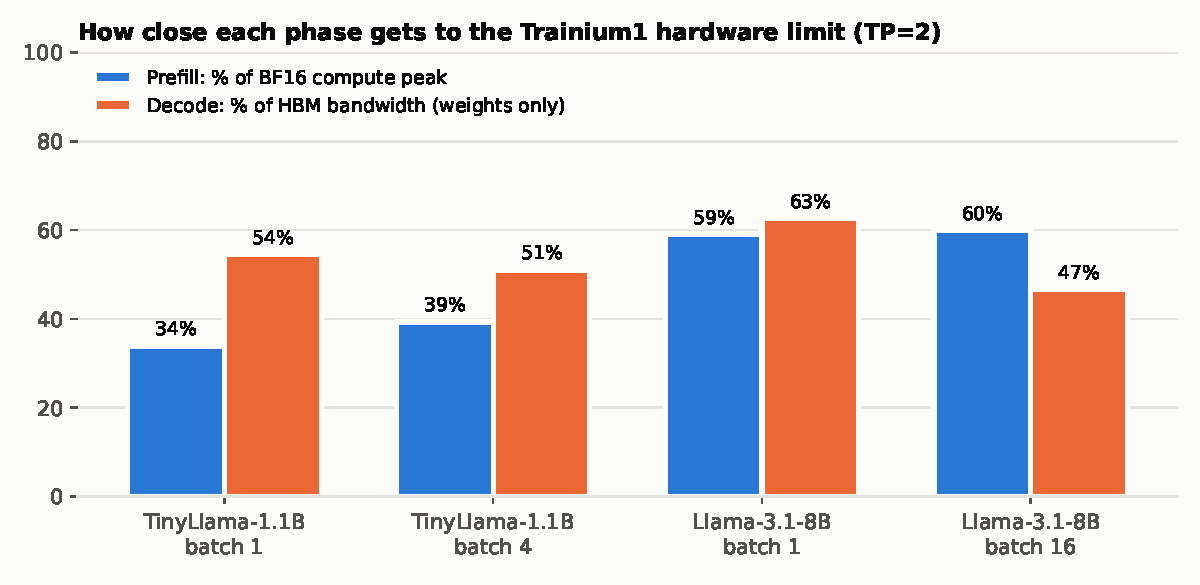
\includegraphics[width=0.92\linewidth]{figs/efficiency.pdf}
\caption{Measured latency as a fraction of each phase's hardware floor, TP=2.}
\label{fig:eff}
\end{figure}

\subsection{Two cores beat one, even for a 1.1B model}
A 1.1B model fits on one NeuronCore, and an early profile showed the TP=2 decode step spending 7--31\% of its time in the
cross-core all-reduce, so we expected TP=1 to decode faster. It did not: TP=2 decodes 1.9$\times$ faster at batch 1 (4.92 vs
9.26\,ms) and prefills 1.4$\times$ faster (Figure~\ref{fig:tp}). With TP=1 the step can use only one core's share of HBM bandwidth
and reaches 29\% of the chip's floor; the collective costs far less than the bandwidth it unlocks.

\begin{figure}[t]
\centering
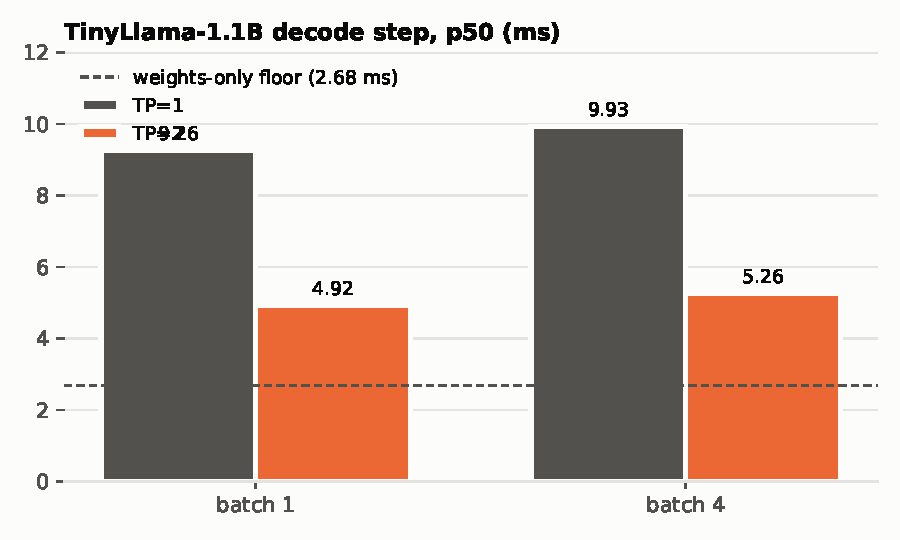
\includegraphics[width=0.62\linewidth]{figs/tp_decode.pdf}
\caption{TinyLlama decode step at TP=1 and TP=2 against the weights-only floor.}
\label{fig:tp}
\end{figure}

\subsection{Batching is nearly free for decode}
Because decode reads the weights once per step regardless of batch size, batching Llama-3.1-8B from 1 to 16 sequences raised decode
throughput from 32 to 381 tokens/s (12$\times$) while the step grew from 31.3 to 42.1\,ms (Figure~\ref{fig:batch}). The weights-only
efficiency drops to 47\% at batch 16 only because the floor ignores the KV cache: 16 sequences averaging about 1536 tokens at
128\,KB per token read about 3.2\,GB per step, which moves the floor to roughly 23.5\,ms and the efficiency to about 56\%.

\begin{figure}[t]
\centering
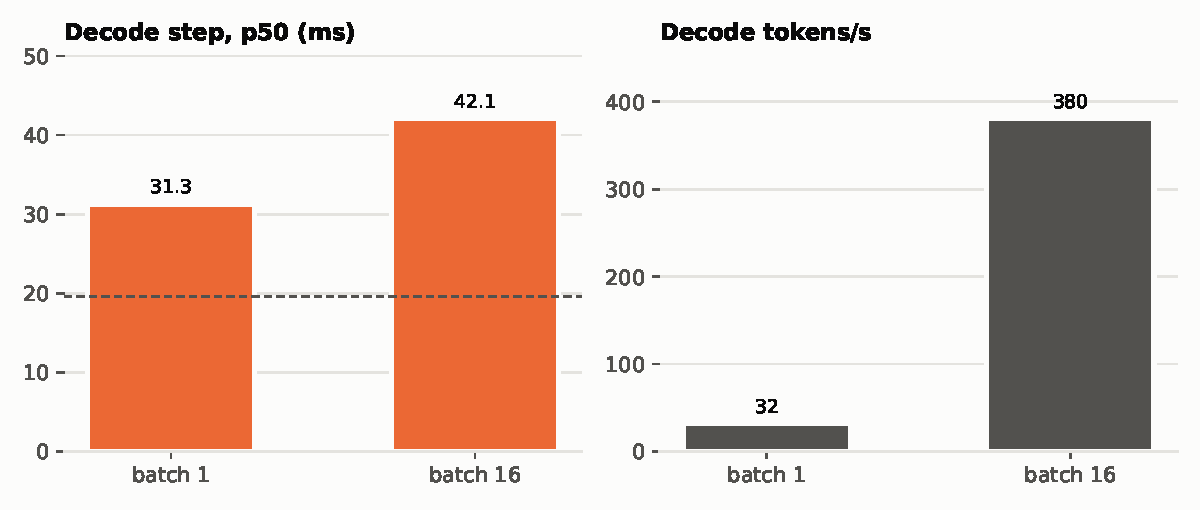
\includegraphics[width=0.8\linewidth]{figs/batching_8b.pdf}
\caption{Llama-3.1-8B, TP=2: decode step time (dashed line: weights-only floor) and decode tokens/s.}
\label{fig:batch}
\end{figure}

\subsection{Where the time goes}
Device profiles of TinyLlama at TP=2, batch 1, show the expected split. In the decode graph, core 0's DMA engines were busy 94\%
of the time while the matrix engine was active about 30\%: the step is streaming weights. Core 1 spent 31\% of its decode time in
collectives and finished later than core 0 (6.3 vs 4.7\,ms in the profiled iteration), so the two cores are not perfectly balanced.
In the prefill graph the matrix engine was active 51--58\% of the time, collectives took about 13\%, vector and scalar engines
20--34\%, and 26\,MB spilled from SBUF. For Llama-3.1-8B we captured only the decode trace of core 0 (31.05\,ms): six DMA queues
were busy for the entire step, again consistent with a weight-streaming bound.

\subsection{Serving overhead}
\begin{table}[t]
\centering
\small
\begin{tabular}{lrrrrr}
\toprule
Concurrency & TTFT p50 (ms) & TTFT p99 (ms) & TPOT p50 (ms) & Output tok/s & Requests/s \\
\midrule
1 & 24.4 & 25.0 & 7.64 & 128 & 1.00 \\
4 & 55.3 & 84.7 & 7.81 & 490 & 3.82 \\
\bottomrule
\end{tabular}
\caption{vLLM 0.13 + \texttt{vllm-neuron} 0.4.1 serving TinyLlama-1.1B at TP=2 (256 tokens in, 128 out, 64 prompts).}
\label{tab:vllm}
\end{table}
Table~\ref{tab:vllm} shows vLLM serving TinyLlama. Time per output token at concurrency 1 was 7.64\,ms, about 55\% above the
4.92\,ms decode step NxDI measured directly. The two numbers come from different harnesses and sequence-length buckets, so this is
an indication rather than a controlled comparison; scheduler and host-side work per step are the likely sources and are not yet
isolated. Four concurrent clients raised throughput 3.8$\times$ with almost no change in time per output token.

\section{Practical notes}
\begin{itemize}
\item \textbf{Pin the SDK.} Neuron 2.29+ dropped Trn1/Inf2 from NxD Inference. Installing NxDI into a newer image pulled a
mismatched \texttt{torch-xla} and broke every step; use the 2.28 DLAMI as shipped.
\item \textbf{Compile elsewhere.} Compiling the 8B model needed 6--9 minutes and 26--28\,GB of host RAM per batch size, which
nearly exhausts a \texttt{trn1.2xlarge}. Compiling on a CPU instance and restoring from S3 removed compilation from the Trainium
budget.
\item \textbf{vLLM flags.} With vLLM 0.13 and \texttt{vllm-neuron} 0.4.1 the server refused to start until prefix caching was
disabled (\texttt{--no-enable-prefix-caching}); setting \texttt{VLLM\_NEURON\_FRAMEWORK} to
\texttt{neuronx-distributed-inference} selects the NxDI backend. Starting one server and sweeping client concurrency avoids recompiling per concurrency level.
\item \textbf{Time budgets.} NxDI's benchmark runs 20 full generations; for the 8B model that took 13--18 minutes per batch size,
and the profile step was cut off by the one-hour budget.
\end{itemize}

\section{Limitations}
Each configuration was measured in one run on one instance, so we cannot report run-to-run variance (within-run p99 was within
1\% of p50). The floors are deliberately simple and optimistic. Only two models and a few batch sizes were measured, all with
NxDI's default kernels; we did not tune bucketing, fuse kernels, or try quantization. The 8B profile is partial, the third graph in
the TinyLlama profile is unidentified, and vLLM was not run on the 8B model. Results are specific to Trainium1 with Neuron 2.28 and
should not be read as representative of Trainium2.

\section{Cost}
Six instance launches (including two that failed early) cost about \$6.0 in compute: roughly \$1.30 for each one-hour
\texttt{trn1.2xlarge} run, \$0.35 for the CPU compile instance, and \$0.35 for a launch stopped by a network misconfiguration.

\section{Conclusion}
On a single Trainium1 chip, an unmodified NxD Inference stack delivers 54--63\% of the bandwidth floor for decode and 34--60\% of
the compute floor for prefill, with larger models closer to the limit. Using both cores and batching are the two largest
levers; both are configuration changes rather than kernel work. The remaining gap---fixed per-step costs for small models,
a constant 40\% overhead in 8B prefill, and serving-layer overhead---is where custom kernels and scheduler work would go next.

\paragraph{Reproducibility.} Scripts, per-run configuration, logs, step exit codes and benchmark reports are at \repo.

\begin{thebibliography}{9}
\bibitem{williams2009roofline}
S.~Williams, A.~Waterman, and D.~Patterson.
\newblock Roofline: an insightful visual performance model for multicore architectures.
\newblock \emph{Communications of the ACM}, 52(4):65--76, 2009.

\bibitem{pope2023efficiently}
R.~Pope, S.~Douglas, A.~Chowdhery, J.~Devlin, J.~Bradbury, et~al.
\newblock Efficiently scaling Transformer inference.
\newblock In \emph{Proceedings of MLSys}, 2023.
\end{thebibliography}

\end{document}
